\documentclass[11pt]{exam}

\usepackage{amsmath, amssymb, amsthm, multicol}
\usepackage{graphicx}
\usepackage{textcomp}
\usepackage{tikz}

\def\d{\displaystyle}
\def\b{\mathbf}
\def\R{\mathbb{R}}
\def\Z{\mathbb{Z}}
\def\N{\mathbb{N}}
\def\pow{\mathcal{P}}
\def\st{~:~}
\def\bar{\overline}
\def\inv{^{-1}}
\def\imp{\rightarrow}
\def\and{\wedge}

\newcommand{\vtx}[2]{node[fill,circle,inner sep=0pt, minimum size=7pt,label=#1:#2]{}}
\newcommand{\va}[1]{\vtx{above}{#1}}
\newcommand{\vb}[1]{\vtx{below}{#1}}
\newcommand{\vr}[1]{\vtx{right}{#1}}
\newcommand{\vl}[1]{\vtx{left}{#1}}
\renewcommand{\v}{\vtx{above}{}}

%\pointname{pts}
\pointsinmargin
\marginpointname{pts}
\addpoints
\pagestyle{head}
%\printanswers

\firstpageheader{Math 228}{\bf Practice Problems 10: Graph Theory \\ Solutions}{Spring 2012}


\begin{document}
 

\begin{questions}

\question This is asking for the number of edges in $K_{10}$.  Each vertex (person) has degree (shook hands with) 9 (people).  So the sum of the degrees is $90$.  However, the degrees count each edge (handshake) twice, so there are 45 edges in the graph.  That is how many handshakes took place.%If 10 people each shake hands with each other, how many handshakes took place?  What does this question have to do with graph theory?

\question It is possible for everyone to be friends with exactly 2 people - you could arrange the 5 people in a circle and say that everyone is friends with the two people on either side of them (so you get the graph $C_5$).  However, it is not possible for everyone to be friends with 3 people - that would lead to a graph with an odd number of odd degree vertices which is impossible - the sum of the degrees must be even.  %Among a group of 5 people, is it possible for everyone to be friends with exactly 2 of the people in the group?  What about 3 of the people in the group?

\question This is a question about finding Euler paths.  Draw a graph with a vertex in each state, and connect vertices if their states share a border.  Exactly two vertices will have odd degree - the vertices for Nevada and Utah.  Thus you must start your road trip at in one of those states and end it in the other. %You and your friends want to tour the southwest by car.  You will visit the nine states below, with the following rather odd rule: you must cross each border between neighboring states exactly once (so, for example, you must cross the Colorado-Utah border exactly once).  Can you do it?  If so, does it matter where you start your road trip?  What fact about graph theory solves this problem?

%\centerline{\includegraphics[height=1in]{images/southwest_map.png}}

\question The first and the third graphs are the same, but the middle graph is different. %Which (if any) of the graphs below are the same?  Which are different?  Explain.

% \begin{center}
%   \begin{tikzpicture}[yscale=.7]
%     \draw[thick] (-2,0) \v -- (0,0) \v -- (2,0) \v -- (-1,2) \v -- (1,2) \v -- (0,0) -- (-1,2) (1,2) -- (-2,0);
%   \end{tikzpicture}
%   \hfill
%   \begin{tikzpicture}[yscale=.7]
%     \draw[thick] (-2,0) \v -- (0,0) \v -- (2,0) \v -- (0,1) \v -- (-2,0) -- (0,2) \v -- (2,0) (0,2) -- (0,1);
%   \end{tikzpicture}
%   \hfill
%   \begin{tikzpicture}[yscale=1]
%     \draw[thick] (-1, 0) \v -- (-1,1) \v -- (0,1) \v -- (1,1) \v -- (1,0) \v -- (0,1) -- (-1,0);
%     \draw[thick] (-1,1) to [out=60, in=120] (1,1);
%   \end{tikzpicture}
% 
% 
% \end{center}

\question The first (and third) graphs contain an Euler path.  All the graphs are planar. %Which of the graphs in the previous question contain Euler paths or circuits?  Which of the graphs are planar?

\question Yes.  For example, both graphs below contain 6 vertices, 7 edges, and have degrees (2,2,2,2,3,3).
\begin{center}
  \hfill
  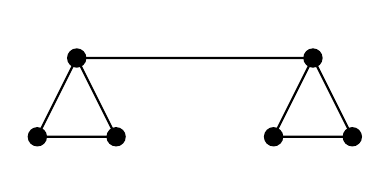
\begin{tikzpicture}
   \draw[thick] (-2,0) \v -- (-1,0) \v -- (-1.5,1) \v -- (-2,0) (-1.5,1) -- (1.5, 1) \v -- (1,0) \v -- (2,0) \v -- (1.5,1);  
  \end{tikzpicture}
  \hfill
  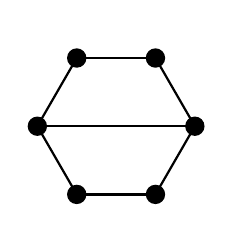
\begin{tikzpicture}
  \foreach \x in {0,...,5}
    \draw[thick] (\x*60:1) \v -- (\x*60 + 60:1);
    \draw[thick] (0:1) -- (180:1);
  \end{tikzpicture}
  \hfill ~
\end{center}


%Is it possible for two {\em different} graphs to have the same number of vertices and the same number of edges?  What if the degrees of the vertices in the two graphs are the same (so both graphs have vertices with degrees 1, 2, 2, 3, and 4, for example)?  Draw two such graphs or explain why not.

\question %Which of the following graphs contain an Euler path?  Which contain an Euler circuit?
\begin{parts}
  \part $K_4$ does not have an Euler path or circuit.
  \part $K_5$ has an Euler circuit (so also an Euler path).
  \part $K_{5,7}$ does not have an Euler path or circuit.
  \part $K_{2,7}$ has an Euler path but not an Euler circuit.
  \part $C_7$ has an Euler circuit (it is a circuit graph!)
  \part $P_7$ has an Euler path but no Euler circuit.
\end{parts}

\question When $n$ is odd, $K_n$ contains an Euler circuit.  This is because every vertex has degree $n-1$, so an odd $n$ results in all degrees being even.%For which $n$ does the graph $K_n$ contain an Euler circuit?  Explain.

\question If both $m$ and $n$ are even, then $K_{m,n}$ has an Euler circuit.  When both are odd, there is no Euler path or circuit.  If one is 2 and the other is odd, then there is an Euler path but not an Euler circuit. %For which $m$ and $n$ does the graph $K_{m,n}$ contain an Euler path?  An Euler circuit?  Explain.

\question Three of the graphs are bipartite.  The one which is not is $C_7$ (second from the right). %Which of the graphs below are bipartite?  
% 
% \begin{center}
%   \begin{tikzpicture}
%     \draw[thick] (-1,1) \v -- (0,2) \v -- (1,1) \v -- (0,0) \v -- (-1,1) -- (0,1) \v -- (1,1);
%   \end{tikzpicture}
%   \hfill
%   \begin{tikzpicture}
%     \draw[thick] (0:1) \v -- (120:1) \v -- (60:1) \v -- (300:1) \v -- (180:1) \v -- (240:1) \v -- cycle;
%   \end{tikzpicture}
%   \hfill
%   \begin{tikzpicture}
%     \draw[thick] (360/7:1) \v -- (2*360/7:1) \v -- (3*360/7:1) \v -- (4*360/7:1) \v -- (5*360/7:1) \v -- (6*360/7:1) \v -- (0:1) \v -- cycle;
%   \end{tikzpicture}
%   \hfill 
%   \begin{tikzpicture}
%     \draw (0,0) \v;
%     \foreach \x in {0,...,7}
%     \draw[thick] (0,0) -- (\x*360/8:1) \v;
%   \end{tikzpicture}
% 
% \end{center}

\question $C_n$ is bipartite if and only if $n = 1$ or is even.%For which $n$ is the graph $C_n$ bipartite?

\question For example, $K_5$. %Draw a graph which has an Euler circuit but is not planar.

\question For example, $K_{3,3}$. %Draw a graph which does not have an Euler path and is also not planar.

\question No.  A (connected) planar graph must satisfy Euler's formula: $V - E + F = 2$.  Here $V - E + F = 6 - 10 + 5 = 1$. %Is it possible for a planar graph to have 6 vertices, 10 edges and 5 faces?  Explain.

\question Yes.  According to Euler's formula it would have 2 faces.  It does.  The only such graph is $C_{10}$. %If a graph has 10 vertices and 10 edges and contains an Euler circuit, must it be planar?  How many faces would it have?

\question $G$ has 10 edges.  It could be planar, and then it would have 6 faces. %The graph $G$ has 6 vertices with degrees $2, 2, 3, 4, 4, 5$.  How many edges does $G$ have?  Could $G$ be planar?  If so, how many faces would it have.

\question 2, since the graph is bipartite.  One color for the top set of vertices, another color for the bottom set of vertices.  %What is the smallest number of colors you need to properly color the vertices of $K_{4,5}$.  That is, find the chromatic number of the graph.

\question For example, $K_6$.  If the chromatic number is 6, then the graph is not planar - the 4-color theorem states that all planar graphs can be colored with 4 or fewer colors. %Draw a graph with chromatic number 6 (i.e., which requires 6 colors to properly color the vertices).  Could your graph be planar?  Explain.

\question The chromatic numbers are 2, 3, 4, 5, and 3 respectively from left to right. %Find the chromatic number of each of the following graphs.
% 
% \begin{center}
%   \begin{tikzpicture}
%     \draw[thick] (-1,1) \v -- (0,2) \v -- (1,1) \v -- (0,0) \v -- (-1,1) -- (0,1) \v -- (1,1);
%   \end{tikzpicture}
%   \hfill
%   \begin{tikzpicture}
%     \draw[thick] (360/7:1) \v -- (2*360/7:1) \v -- (3*360/7:1) \v -- (4*360/7:1) \v -- (5*360/7:1) \v -- (6*360/7:1) \v -- (0:1) \v -- cycle;
%   \end{tikzpicture}
%   \hfill 
%   \begin{tikzpicture}
%     \draw (0,0) \v;
%     \foreach \x in {0,...,4}
%     \draw[thick] (0,0) -- (\x*360/5:1) \v -- (\x*360/5+72:1);
%   \end{tikzpicture}
%   \hfill
%   \begin{tikzpicture}
%     \foreach \x in {0,...,4}
%     \draw[thick] (\x*72+18:1) \v -- (\x*72+90:1) -- (\x*72-54:1);
%   \end{tikzpicture}
%   \hfill
%     \begin{tikzpicture}[scale=.6]
%     \draw[thick] (18:2) -- (90:2) -- (162:2)  -- (234:2) -- (306:2) -- cycle; 
%     \draw[thick] (18:1) --  (162:1)  -- (306:1) -- (90:1) -- (234:1) --cycle;
%     \foreach \x in {18, 90, 162, 234, 306}
%     \draw[thick] (\x:1) \v -- (\x:2) \v;
%   \end{tikzpicture}
% \end{center}

\question %Suppose $G$ is a simple graph with $n$ vertices, each having degree 5. 
\begin{parts}
  \part Only if $n \ge 6$ and is even.%For which values of $n$ does this make sense?
  \part None. %For which values of $n$ does the graph have an Euler path?
  \part 12. Such a graph would have $\frac{5n}{2}$ edges.  If the graph is planar, then $n - \frac{5n}{2} + F = 2$ so there would be $\frac{4+3n}{2}$ faces.  Also, we must have $3F \le 2E$, since the graph is simple.  So we must have $3\frac{4 + 3n}{2} \le 5n$.  Solving for $n$ gives $n \ge 12$.%What is the smallest value of $n$ for which the graph might be planar? (tricky)
\end{parts}


\end{questions}


\end{document}


